\section{User model} 
\label{sec:user_model}

We consider many users owning several devices, that they freely turn on and off depending on their location and will.
The participants' devices are the only nodes constituting our system; the unreliability of their connectivity has to be taken for granted.

We will first present a model of each user's behavior, that will drive the connection intervals of our system's nodes.
%Then, we will show how devices can predict the future user's behavior given the model.

\subsection{A model of the user's behavior}
\label{sub:a_model_of_the_user_s_behavior}

In \name, we take interest in users that own several devices, and wish to privately exchange files with each other without revealing .
To the best of our knowledge, no real-world traces of multi-devices usage over several days exist, as would be needed for the experimental evaluation of our system.
For that reason, we propose a user behavioral model having the following features:

\begin{itemize}
	\item Each user owns a variable amount of devices. We consider the following device types: mobile, portable, fixed, and server;
	\item The user travels between three ``locations'' according to a simple probabilistic model: her home, her workplace, and outside;
	\item She makes a different use of her devices depending on her location: at home, she will her laptop that at work; she cannot use her workstation at home.
\end{itemize}

To this end, we use a Hidden Markov Model (HMM) of order one, with multiple discrete observation processes. 
The hidden Markovian process $S$ represents the user's locations, while the \emph{observable} process $O=O_1, \dots, \O_T$ represents the connection state of her devices (either connected or disconnected at any point in time).
% The \emph{hidden} Markovian process $S=S_1,\dots,S_T$ represents the user's progression among the three proposed locations up to time step $T$.
% For every device $d$ owned by the user, the \emph{observable} process $O_d=O_{d,1},\dots,O_{d,T}$ reads $d$'s state: it is either online ($o_d$) or offline ($\overline{o_d}$) at each point in time. $O_t = O_1, \dots, \O_T$ represents the connection of all the user's devices, such that $o_d \in O_t$ means that device $d$ was connected at time $t$.

% The probability of observable events depends only on the current location.
% For example, the probability that the user's home computer is on while she is at work is null (in our model, users never forget to turn off their fixed devices before leaving).

Such a statistical model is simplistic (e.g. it does not encapsulate date \& time nor location), but it is on purpose: simplicity is bliss.
Given the lack of real-world data for our testbed, building a more complex and realistic user model would add no value to our proposal: 
our goal is to see devices exhibiting frequent disconnections and reconnections (also called \emph{churn}).
Our simple model being able to put extravagant stress on our system, it is sufficient to access \name's resilience.

\subsubsection{Formal definition} % (fold)
\label{ssub:formal_definition}


\begin{figure}[t]
\centering
\vspace{-1em}

$$A =
\kbordermatrix{
      & W            & O            & H            \cr
    W & \sfrac{2}{3} & \sfrac{1}{3} & 0            \cr
    O & \sfrac{1}{3} & \sfrac{1}{3} & \sfrac{1}{3} \cr
    H & 0            & \sfrac{1}{3} & \sfrac{2}{3} \\[0.3em]
}, \;
B = 
\kbordermatrix{
      & W     & O   & H   \cr
    o_p & 0.7 & 0.6 & 0.8 \cr
    o_w & 0.7 & 0   & 0   \cr
    o_h & 0   & 0   & 0.7 \cr
    o_l & 0.2 & 0.4 & 0.6 \\[0.3em]
}$$

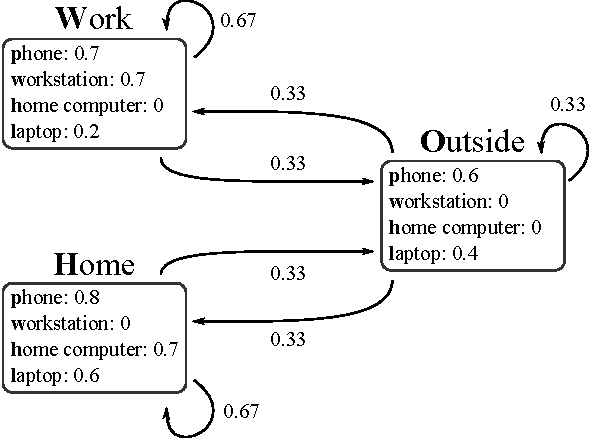
\includegraphics[width=0.9\columnwidth]{figures/hmm.pdf}
\caption{ \label{fig:hmm} Example Hidden Markov Model (HMM) of a user's behavior.}
\end{figure}

We consider a single user, owning a set of $\mathcal{D}$ devices.
Time is discretized \commentAL{Discretized/synchronous time needs more explanation}. Needs, and the devices' observations are independent: Alice can have her laptop and phone connected at the same time.
The hidden process $S=S_1,\dots,S_T$ is built from an alphabet of states $\mathcal{S}$, while the observable process $O=O_1, \dots, \O_T$ contains events from the alphabet $\mathcal{O}$. We define a multivariate HMM $\lambda_N$ as follows:

$$\text{HMM}:\;\lambda_N=(\Pi, A, B)$$

where 
\begin{itemize}
	\item $N$ is the number of states in the system:
	$N = \left| \mathcal{S} \right|$;

	\item $\Pi=\left\{ \pi_i\right\}_{i\in\mathcal{S}}$ is the initial state distribution:\\
	$\pi_i=P[S_1=i]$;

	\item $A = \left\{ a_{i\,j}\right\}_{(i,j)\in\mathcal{S}^2}$ is the state transition matrix:\\
	$a_{i\,j}=P[S_t=j \mid S_{t-1}=i]$;

	\item $B = \left\{ b_{i\,k}\right\}_{(i,k)\in\mathcal{S}\times\mathcal{O}}$ is the matrix of event emission probabilities for each state:
	$b_{i\,k} = P[ k \in O_t \mid S_t = i]$.
\end{itemize}

In our case, the states are the different locations where the user is susceptible to go;
we considered the three following ones: $\mathcal{S}=\left\{ \mathit{work}, \mathit{outside}, \mathit{home} \right\}$. 
There is one event per device $d$: $\mathcal{O} = \left\{ o_d \right\}_{d\in \mathcal{D}}$. Several devices can be connected at the same time, such that $O_t$ is a set, and $o_d \in O_t$ means that device $d$ was connected at time $t$. Devices' connection probabilities are independent.

In \cref{fig:hmm}, we show an example HMM of a user's behavioral HMM, along with its graphical representation (the initial state distribution $\Pi$ was left out for simplicity). 
The represented user possesses a phone and a laptop, that she carries around with her, a home computer, that is only accessible from her home, and a workstation, located at her workplace. She never forgets to turn off her fixed appliances before leaving.

\begin{figure}[t]
\centering
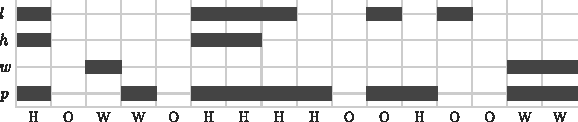
\includegraphics[width=\columnwidth]{figures/sample_usage.pdf}

\caption{\label{fig:sample_usage}Sample device usages using the previous HMM specifications. 
%The bottom line reads the HMM's states: \textbf{W}ork, \textbf{O}utside, and \textbf{H}ome, while the dark lines read when the devices (\textbf{h}ome computer, \textbf{p}hone, and \textbf{w}orkstation) are online.
}

\end{figure}

% Using the toggle events, we compute the device's \emph{connection} events, represented by the multivariate Bernoulli process $C=\left\{ c^{(d)} \right\}_{d\in\mathcal{D}}$. 
% $c^{(d)}_t=1$ (resp. 0) means that the device $d$ was online (resp. offline) at time step $t$.

% We state that every device starts offline, and compute $c^{(d)}_t$ as follows:

% $$ \forall d \in \mathcal{D},
% \begin{cases}
% c^{(d)}_t=0 &\text{when } t=0; \\
% c^{(d)}_t=c^{(d)}_{t-1} \oplus o^{(d)}_t &\text{when } t>0.
% \end{cases}$$

Figure~\ref{fig:sample_usage}, shows a possible trace of the user's behavior, using the parameters depicted in figure~\ref{fig:hmm}. 
It reads the timeline of $o_{d}$ for each device $d$. On the bottom of the graph, the first letter of the user's location is shown at each time step.
We see that devices connections depend on the user's location, and that any number of devices can be connected at the same time.

% Each device starts offline; then, the user either toggles one device per round or does nothing.
% In this figure, we show the device \emph{usage}, that is a consequence of the $\mathit{toggle}$ events defined by the HMM.
% As a consequence, several devices can be online at the same time, as happens in the figure.

% subsubsection formal_definition (end)


\subsubsection{Predicting future behavior} % (fold)
\label{ssub:predicting_future_behavior}
Devices want to predict whether they are likely to be connected in the near future.
This information will be publicly available, and will allow routes selection for the  files exchange between users.

Because devices connections only depend on the users location, we can predict the devices connections in $i$ round $O_{t+i}$ given only the model $\lambda_N$ and the current user's location $S_t$. We first compute the probability that a device $d$ will be connected next turn:

$$
P\left[ o_d \in O_{t} \mid S_{t-1} = s \right] = 
\sum\limits_{s' \in \mathcal{S}} 
a_{s\,s'} * b_{s'\,o_d}.
$$

It is the sum of the probabilities, for each state $s$, that the user switches to $s$ and uses her device.
\commentAL{Following maybe not needed if we only use $t+1$:}
Recursively, predicting $i$ turns in advance follows the same logic:

\begin{multline*}
P\left[ o_d \in O_{t+i} \mid S_{t} = s \right] = \\
\sum\limits_{s' \in \mathcal{S}}
P\left[ S_{t+1} = s' \mid S_t = s \right] * 
P\left[ o_d \in O_{t+i} \mid S_{t+1} = s'\right].
\end{multline*}


\commentAL{In conclusion: we want more unicorns at the Olympic Games.}

\commentAL{I don't mention prediction yet since I am not sure we get good enough results.}